\documentclass[12pt,letterpaper]{article}

\usepackage[spanish,es-tabla]{babel}
\usepackage[utf8]{inputenc}
\usepackage[T1]{fontenc}
\usepackage{lmodern}
\usepackage{geometry}
\usepackage{setspace}
\usepackage{graphicx}
\usepackage{booktabs}
\usepackage{longtable}
\usepackage{float}
\usepackage{hyperref}
\usepackage{caption}
\usepackage{enumitem}
\usepackage{fancyhdr}
\usepackage{microtype}
\usepackage{parskip}

\geometry{margin=2.54cm}
\setstretch{1.5}
\captionsetup[table]{skip=6pt}
\captionsetup[figure]{skip=6pt}
\hypersetup{
  colorlinks=true,
  linkcolor=blue,
  urlcolor=blue,
  citecolor=blue,
  pdftitle={Informe final consultoria de Minciencias},
  pdfauthor={Maria Paula Amaya y Paula Andrea Betancour}
}

\pagestyle{fancy}
\fancyhf{}
\fancyhead[L]{Informe final consultoria}
\fancyhead[R]{Minciencias}
\fancyfoot[C]{\thepage}

\graphicspath{{imagenes/}}

\begin{document}

\begin{titlepage}
    \centering
    {\Large Universidad Santo Tomas\par}
    \vspace{0.4cm}
    {\large Consultoria e Investigacion Ustadistica\par}
    \vspace{1.7cm}
    {\LARGE \textbf{Informe final consultoria de Minciencias}\par}
    \vspace{1.0cm}
    {\large Proyecto: Observatorio MinCiencias - Investigadores Reconocidos\par}
    \vspace{0.9cm}
    {\large Integrantes: Maria Paula Amaya y Paula Andrea Betancour\par}
    \vspace{0.35cm}
    {\large Docente: Carlos Isaac Zainea\par}
    \vspace{0.35cm}
    {\large Ano: 2026\par}
    \vfill
\end{titlepage}

\tableofcontents
\newpage

\section{Resumen}

Este informe presenta de manera ordenada y comprensible el proceso completo de la consultoria realizada sobre convocatorias de investigadores reconocidos por Minciencias. La intencion fue construir un trabajo reproducible, util para analisis territorial y con una salida final clara para visualizacion en linea.

El desarrollo no se limito a crear un dashboard. Primero se organizaron fuentes, luego se consolidaron bases, despues se calcularon indicadores y finalmente se construyo una aplicacion interactiva para consultar resultados por region y convocatoria. En el cierre del proyecto se dejo un tablero funcional que carga datos procesados desde el repositorio, lo cual evita dependencia de archivos locales y facilita validacion por terceros.

Como resultado final se integraron 15 indicadores regionales. Entre los hallazgos mas relevantes se observa el liderazgo sostenido de Distrito Capital en volumen y participacion de produccion, y al mismo tiempo se identifican fortalezas diferenciales en otras regiones para indicadores de permanencia, renovacion y crecimiento.

\textbf{Palabras clave:} Minciencias, indicadores regionales, analitica territorial, dashboard, reproducibilidad.

\section{Introduccion}

El proyecto surge de la necesidad de analizar las convocatorias de investigadores reconocidos de Minciencias con una mirada que combine calidad tecnica y capacidad de comunicacion. Durante el proceso se identifico que no era suficiente calcular metricas de forma aislada: tambien era necesario consolidar una estructura de trabajo que permitiera revisar resultados, explicar decisiones metodologicas y comunicar hallazgos de forma visual.

Por esta razon, el equipo abordo el proyecto en etapas. Primero se trabajo la organizacion del repositorio y la estandarizacion de carpetas de datos, codigo y evidencias. Despues se avanzo en transformaciones de datos y calculo de indicadores. Finalmente se integro todo en una visualizacion interactiva en Streamlit para apoyar la lectura regional de resultados.

\section{Objetivos}

\subsection{Objetivo general}

Desarrollar un proceso analitico reproducible para estudiar el comportamiento regional de la produccion cientifica asociada a Minciencias, y presentar los resultados en un informe academico y en un dashboard web funcional.

\subsection{Objetivos especificos}

\begin{enumerate}[label=\arabic*.]
  \item Consolidar y depurar insumos de datos para trabajar con una base consistente.
  \item Calcular indicadores regionales comparables para diferentes dimensiones del desempeno.
  \item Construir una salida de visualizacion que permita filtrar por convocatoria y region.
  \item Documentar de forma academica el proceso, las decisiones tomadas y los principales resultados.
\end{enumerate}

\section{Metodologia de trabajo}

La metodologia se desarrollo en cuatro momentos:

\begin{enumerate}[label=\arabic*.]
  \item \textbf{Organizacion y diagnostico:} revisamos estructura del repositorio, ubicacion de fuentes y trazabilidad de evidencias.
  \item \textbf{Transformacion de datos:} consolidamos bases y generamos salidas procesadas para analisis.
  \item \textbf{Construccion de indicadores:} calculamos metricas regionales y archivos de salida en formato CSV.
  \item \textbf{Visualizacion y validacion:} integramos los resultados en el dashboard final y verificamos lectura de datos desde rutas versionadas.
\end{enumerate}

Este enfoque permitio que cada resultado del tablero se respaldara en archivos procesados concretos y en evidencia de ejecucion del proyecto.

\section{Proceso realizado paso a paso}

\subsection{Fase 1: organizacion del trabajo}

Al inicio, se priorizo ordenar el proyecto para evitar dispersion de archivos. Se definieron carpetas con funciones claras: datos, codigo fuente, documentacion y hallazgos. Esta fase fue clave porque permitio que el trabajo posterior no dependiera de rutas personales ni de archivos sueltos.

\subsection{Fase 2: consolidacion y preparacion de datos}

Con la estructura ya definida, se ejecutaron scripts de consolidacion y filtrado para obtener conjuntos procesados estables. El resultado de esta etapa fue disponer de archivos listos para analisis y de salidas intermedias verificables, tanto en formato parquet como en CSV de indicadores.

\subsection{Fase 3: construccion de indicadores regionales}

Con la base consolidada se calcularon indicadores para medir volumen, participacion, intensidad de produccion por grupo, diversidad, permanencia, crecimiento y composicion por clasificacion. Esta fase permitio pasar de datos crudos a resultados comparables por region y, cuando aplica, por convocatoria.

\subsection{Fase 4: integracion en dashboard final}

Luego se implemento el tablero final en Streamlit con dos archivos principales de aplicacion. El primero concentra la interfaz y componentes visuales; el segundo organiza la logica de carga de datos y definicion de metricas. La decision tecnica mas importante fue fijar la ruta de lectura en \texttt{datos/processed/indicadores}, para que el tablero funcionara en linea sin depender de archivos locales.

\subsection{Fase 5: validacion y cierre}

Como cierre, se verifico que el dashboard cargara todos los indicadores esperados y que las salidas fueran coherentes con los CSV finales. De esta manera, el informe y la aplicacion quedaron alineados: lo que se reporta aqui corresponde a resultados realmente versionados en el repositorio.

\section{Arquitectura del producto final}

\subsection{Componentes principales}

\begin{itemize}
  \item Archivo principal de interfaz: \texttt{app/dashboard\_streamlit\_v2.py}
  \item Modulo base de metricas y carga de datos: \texttt{app/dashboard\_streamlit\_final.py}
  \item Datos de entrada del tablero: \texttt{datos/processed/indicadores/*.csv}
  \item Insumos geograficos versionados: \texttt{datos/processed/co.json} y \texttt{datos/processed/co\_shp.zip}
\end{itemize}

\subsection{Indicadores integrados}

El tablero final incluye 15 indicadores regionales. Esta seleccion ofrece una lectura completa del sistema: combina indicadores de volumen, estructura y dinamica temporal.

\section{Resultados}

\subsection{Resumen de liderazgo regional por indicador}

\begin{longtable}{p{7.8cm}p{3.5cm}r}
\toprule
\textbf{Indicador} & \textbf{Region lider} & \textbf{Valor} \\
\midrule
\endfirsthead
\toprule
\textbf{Indicador} & \textbf{Region lider} & \textbf{Valor} \\
\midrule
\endhead
1. Produccion total por region & Distrito Capital & 413229 \\
2. Participacion regional & Distrito Capital & 33.3021 \\
3. Produccion promedio por grupo & Caribe & 235.1502 \\
4. Produccion por clasificacion & Distrito Capital & 413229 \\
5. Diversificacion de productos & Distrito Capital & 75 \\
6. IEP & Caribe & 1.1947 \\
7. Diversidad relativa & Distrito Capital & 98.6842 \\
8. Permanencia de grupos & Caribe & 67.2875 \\
9. Crecimiento neto 2017-2021 & Llano & 69.0909 \\
10. Fortaleza A1/A 2021 & Eje Cafetero & 44.6103 \\
11. Tasa de renovacion & Llano & 53.7634 \\
12. Distribucion por genero (mapa) & Eje Cafetero & 138849 \\
13. Evolucion de grupos 2017-2021 & Caribe & 76.4906 \\
14. Participacion por clasificacion & Centro Oriente & 20 \\
15. Participacion por clasificacion y convocatoria & Llano & 21.4286 \\
\bottomrule
\end{longtable}

\subsection{Produccion nacional por convocatoria}

\begin{table}[H]
\centering
\begin{tabular}{lr}
\toprule
\textbf{Convocatoria} & \textbf{Produccion total} \\
\midrule
2017 & 271924 \\
2019 & 444448 \\
2021 & 524478 \\
\bottomrule
\end{tabular}
\caption{Produccion total nacional por convocatoria.}
\end{table}

\subsection{Lectura de resultados}

El comportamiento general muestra que Distrito Capital mantiene liderazgo en volumen y participacion de produccion. No obstante, el analisis por indicador permite ver matices importantes: Caribe resalta en permanencia e intensidad promedio, Llano en dinamica de crecimiento y renovacion, y Eje Cafetero en fortaleza relativa A1/A. Esto confirma que la lectura territorial mejora cuando se analizan varias dimensiones al mismo tiempo y no solo los totales absolutos.

\subsection{Resultados del mapa del dashboard\_streamlit\_v2 (corte 2021)}

Para complementar la tabla de indicadores, se genero una visualizacion equivalente al mapa regional del dashboard para la metrica de produccion total en 2021. La produccion nacional observada en este corte fue de 524478 productos. En esta lectura, la region con mayor volumen fue Distrito Capital (168771), seguida por Eje Cafetero (117333) y Caribe (85171).

Para tener una lectura temporal completa, tambien se construyeron las mismas visualizaciones para 2017 y 2019. En 2017 la produccion nacional fue de 271924 y en 2019 subio a 444448. En ambos anos se mantiene el mismo patron de liderazgo regional: Distrito Capital, Eje Cafetero y Caribe.

\begin{figure}[H]
  \centering
  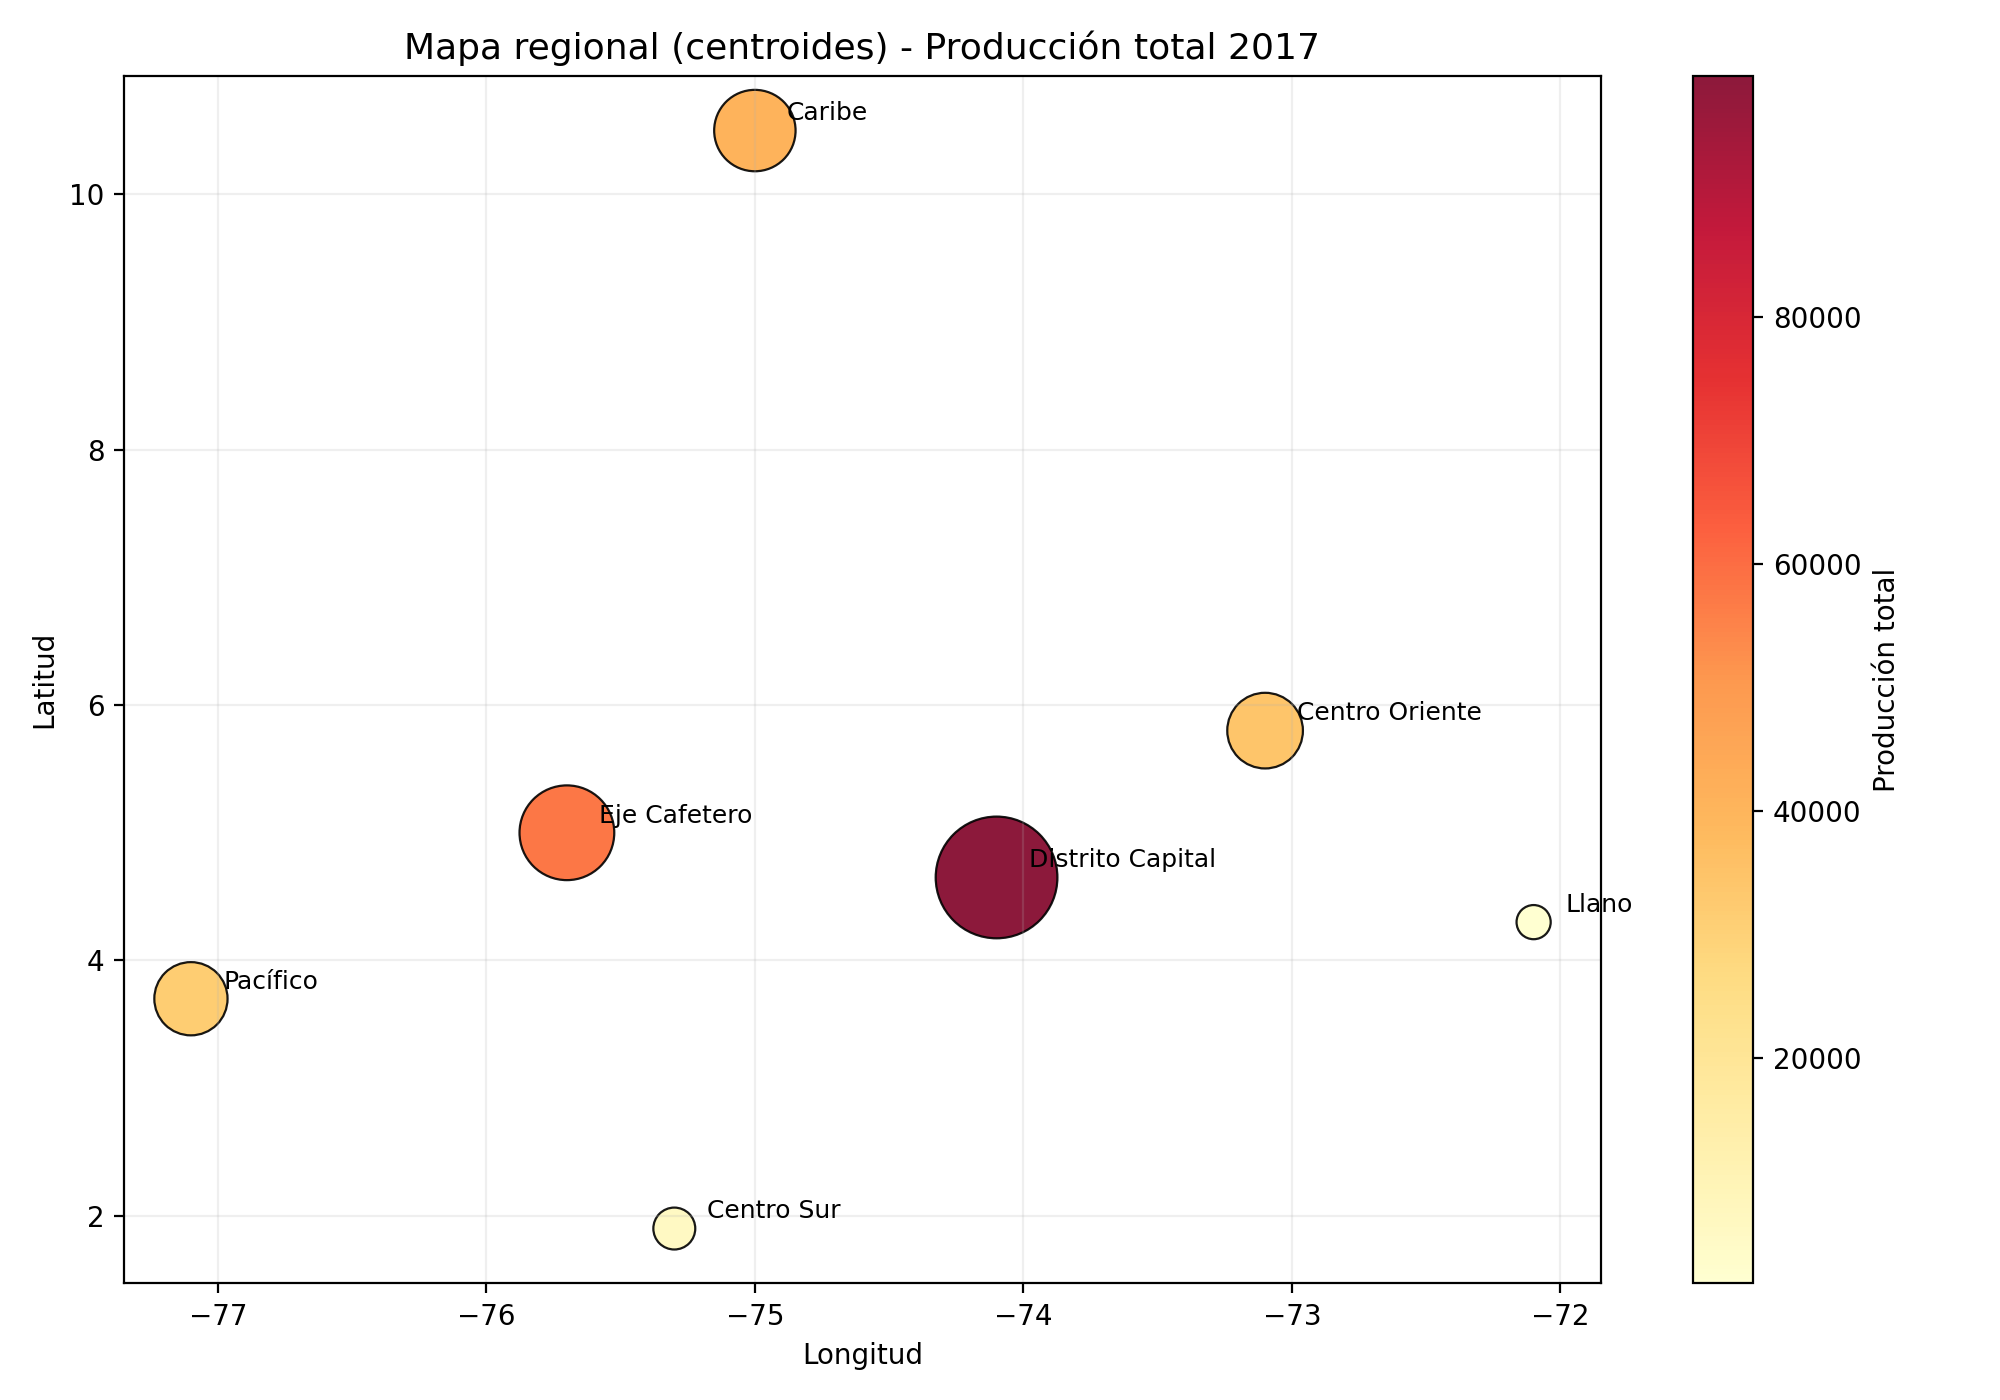
\includegraphics[width=0.88\textwidth]{dashboard_mapa_produccion_2017.png}
  \caption{Mapa regional por centroides para produccion total en 2017.}
\end{figure}

\begin{figure}[H]
  \centering
  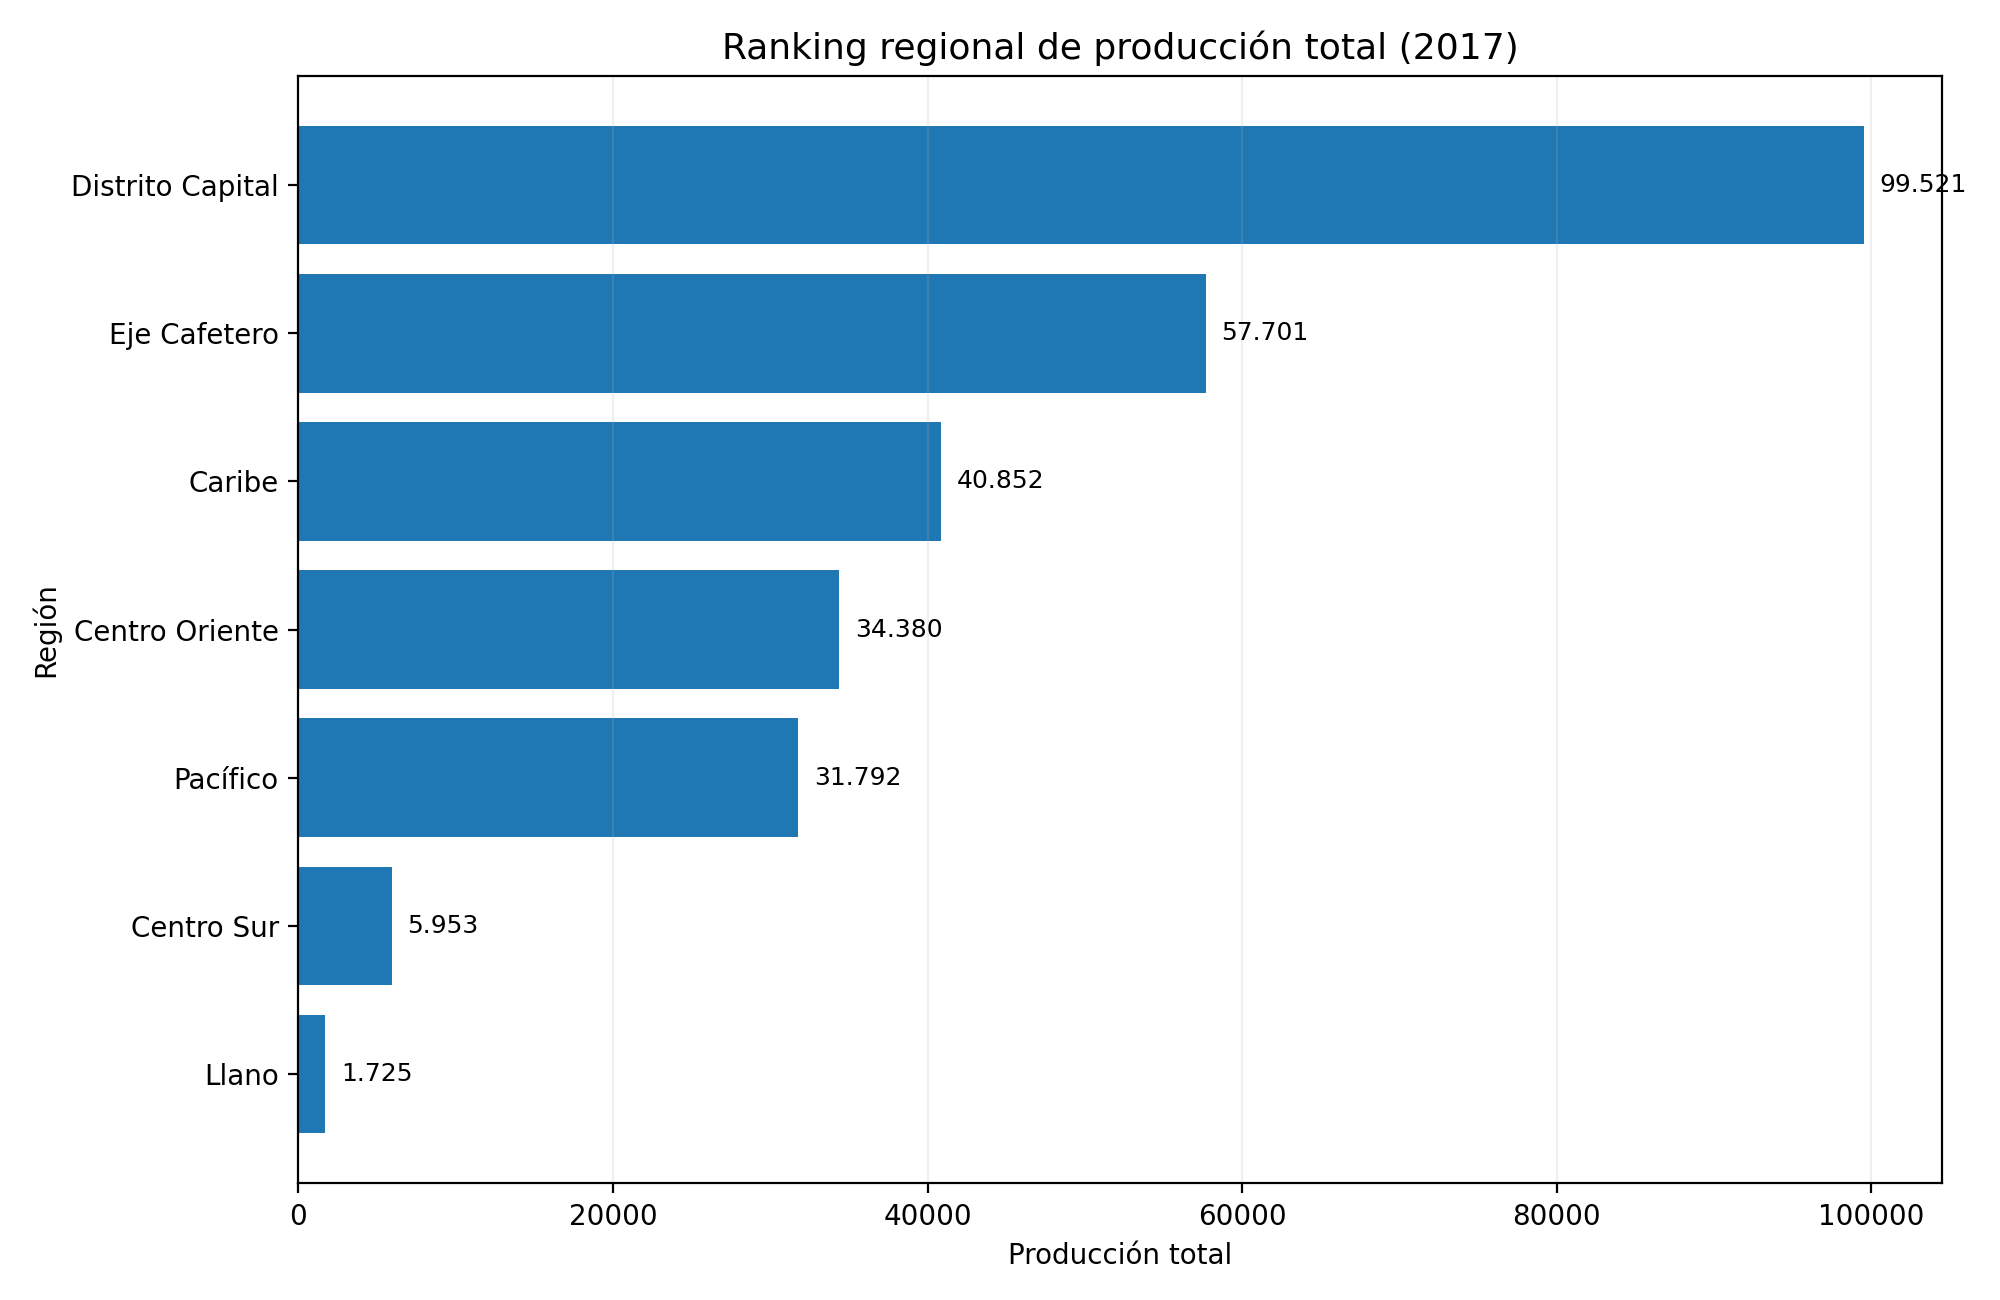
\includegraphics[width=0.88\textwidth]{dashboard_ranking_produccion_2017.png}
  \caption{Ranking regional de produccion total en 2017.}
\end{figure}

\begin{figure}[H]
  \centering
  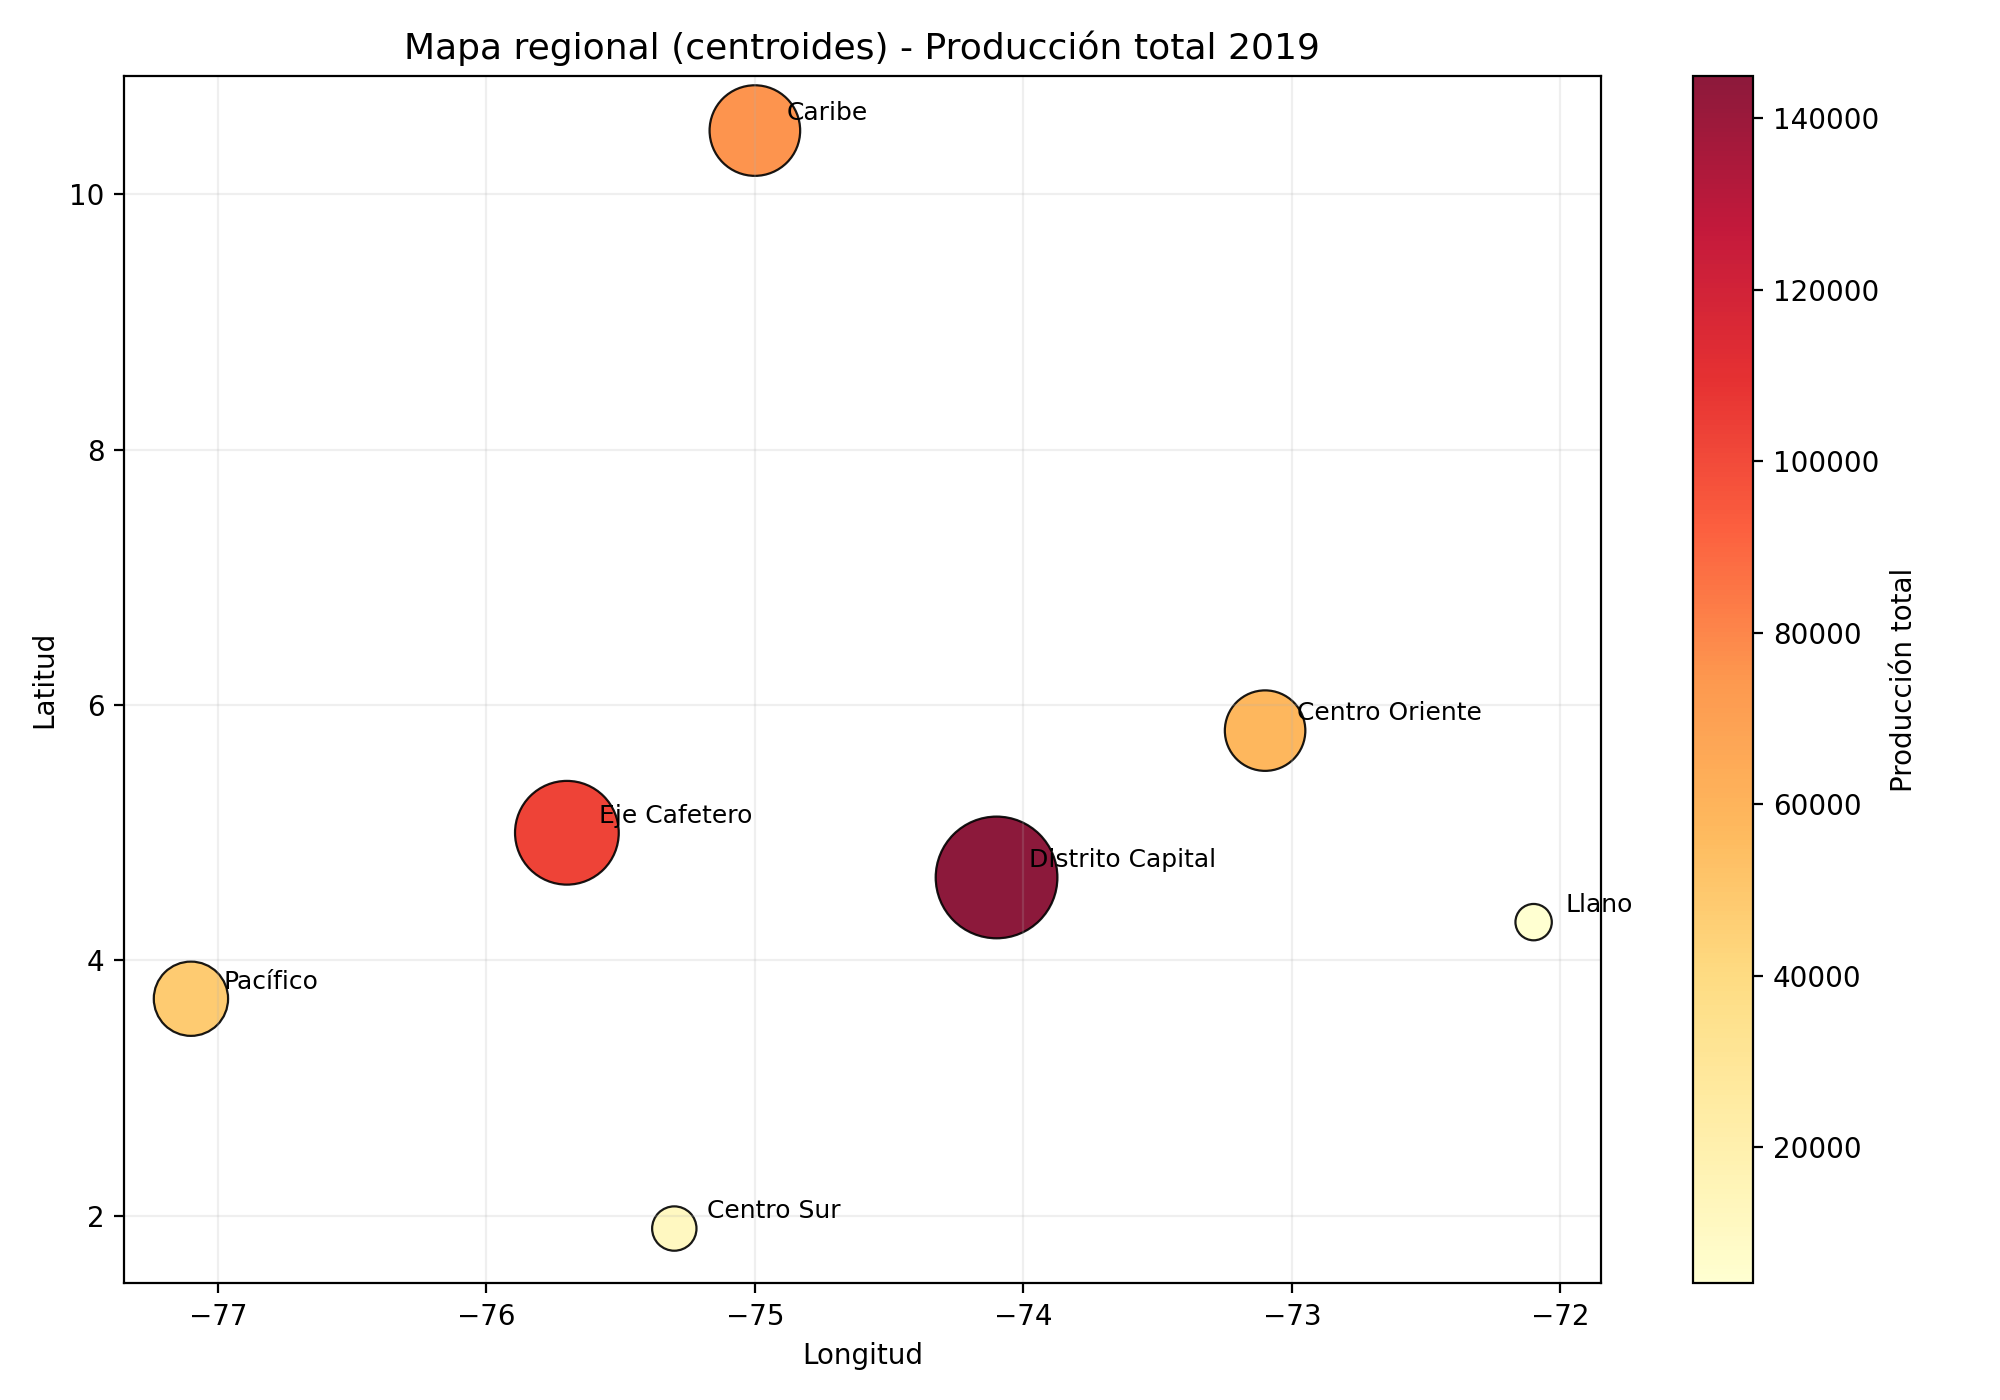
\includegraphics[width=0.88\textwidth]{dashboard_mapa_produccion_2019.png}
  \caption{Mapa regional por centroides para produccion total en 2019.}
\end{figure}

\begin{figure}[H]
  \centering
  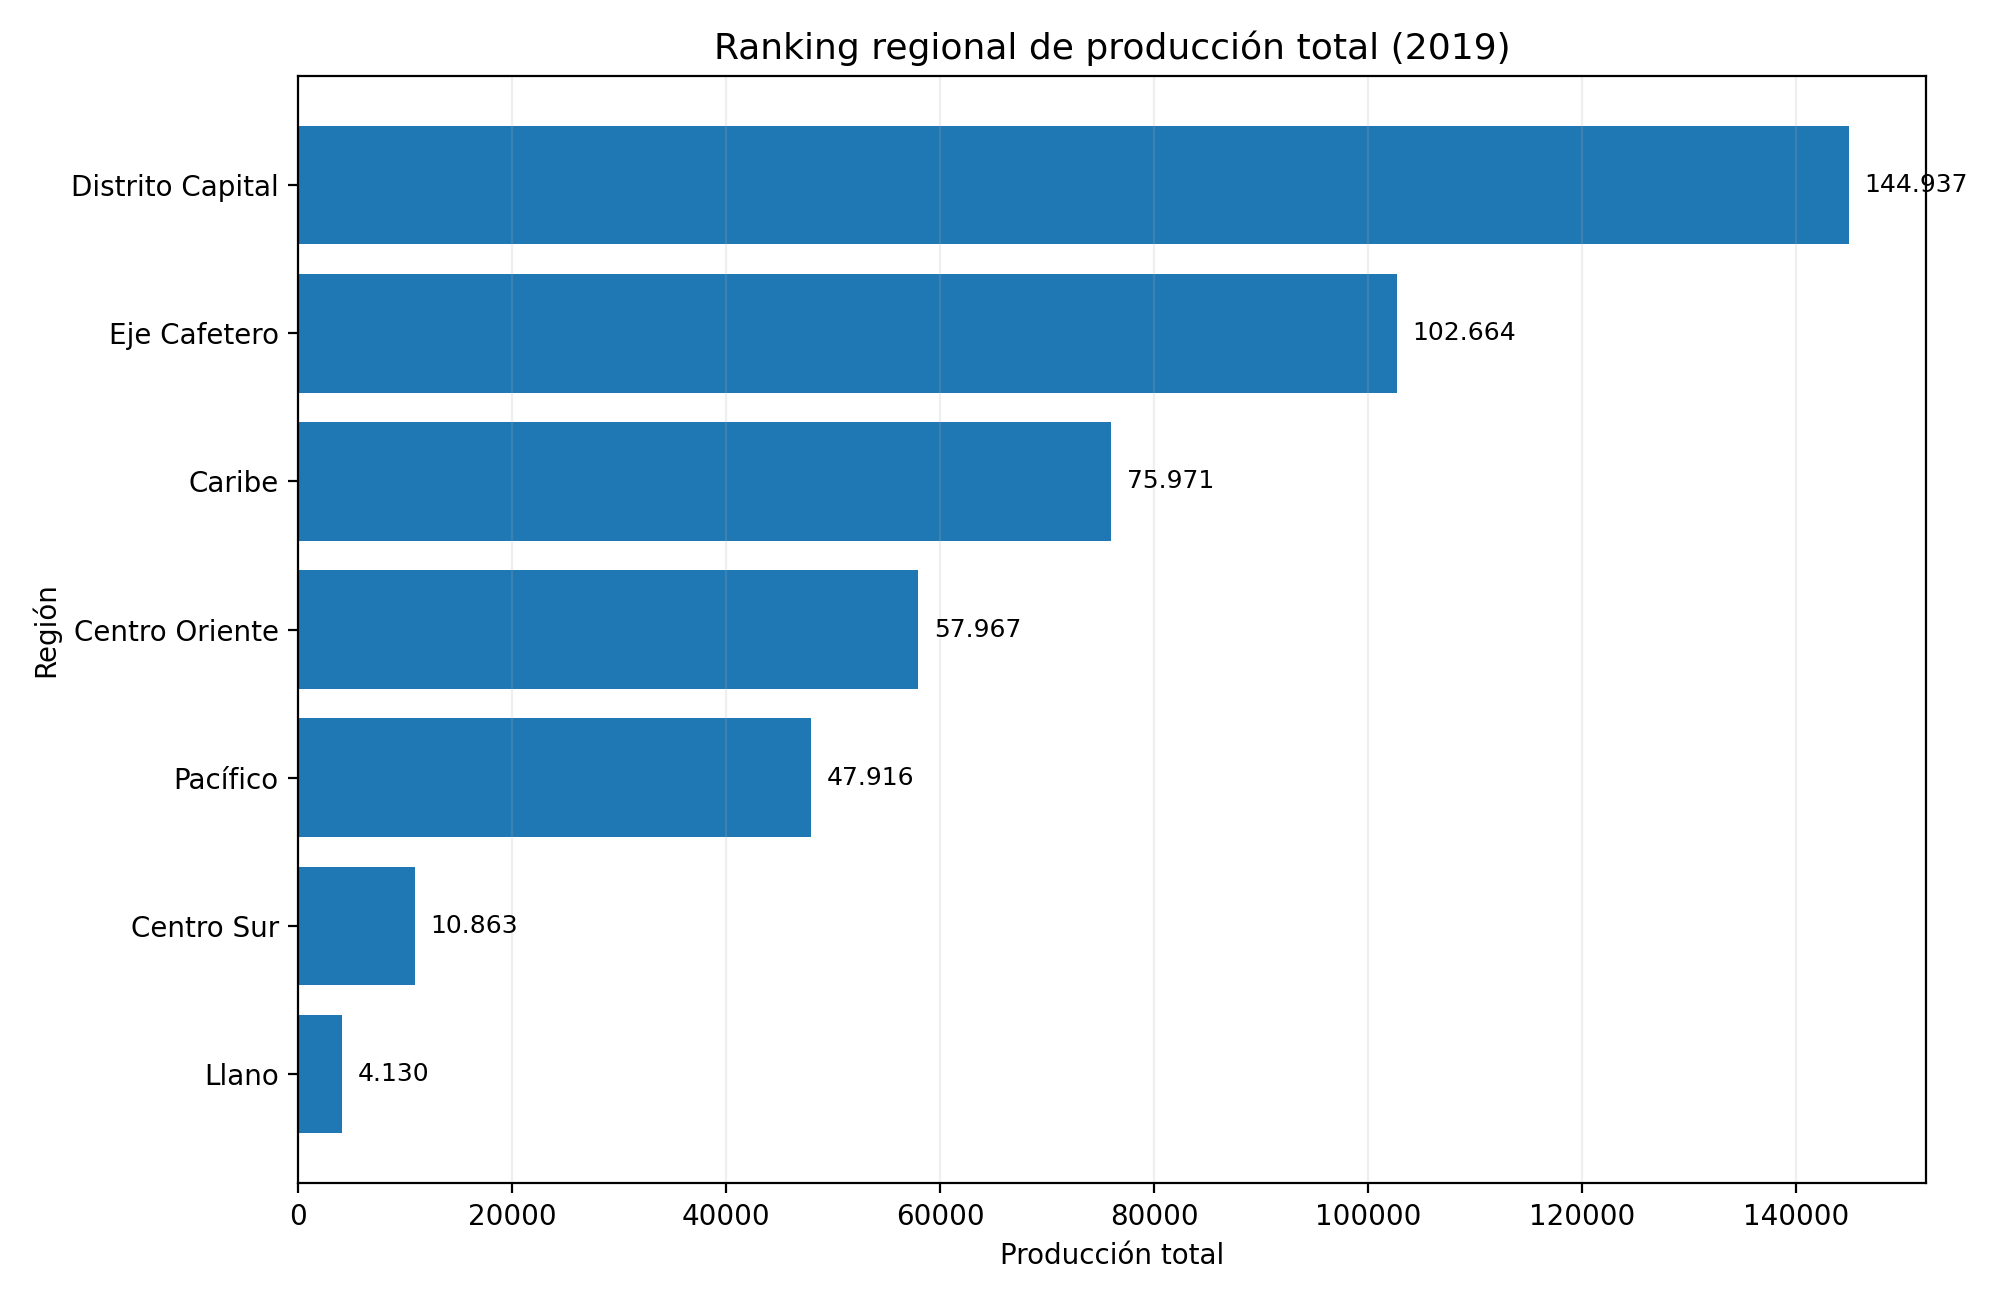
\includegraphics[width=0.88\textwidth]{dashboard_ranking_produccion_2019.png}
  \caption{Ranking regional de produccion total en 2019.}
\end{figure}

\begin{figure}[H]
  \centering
  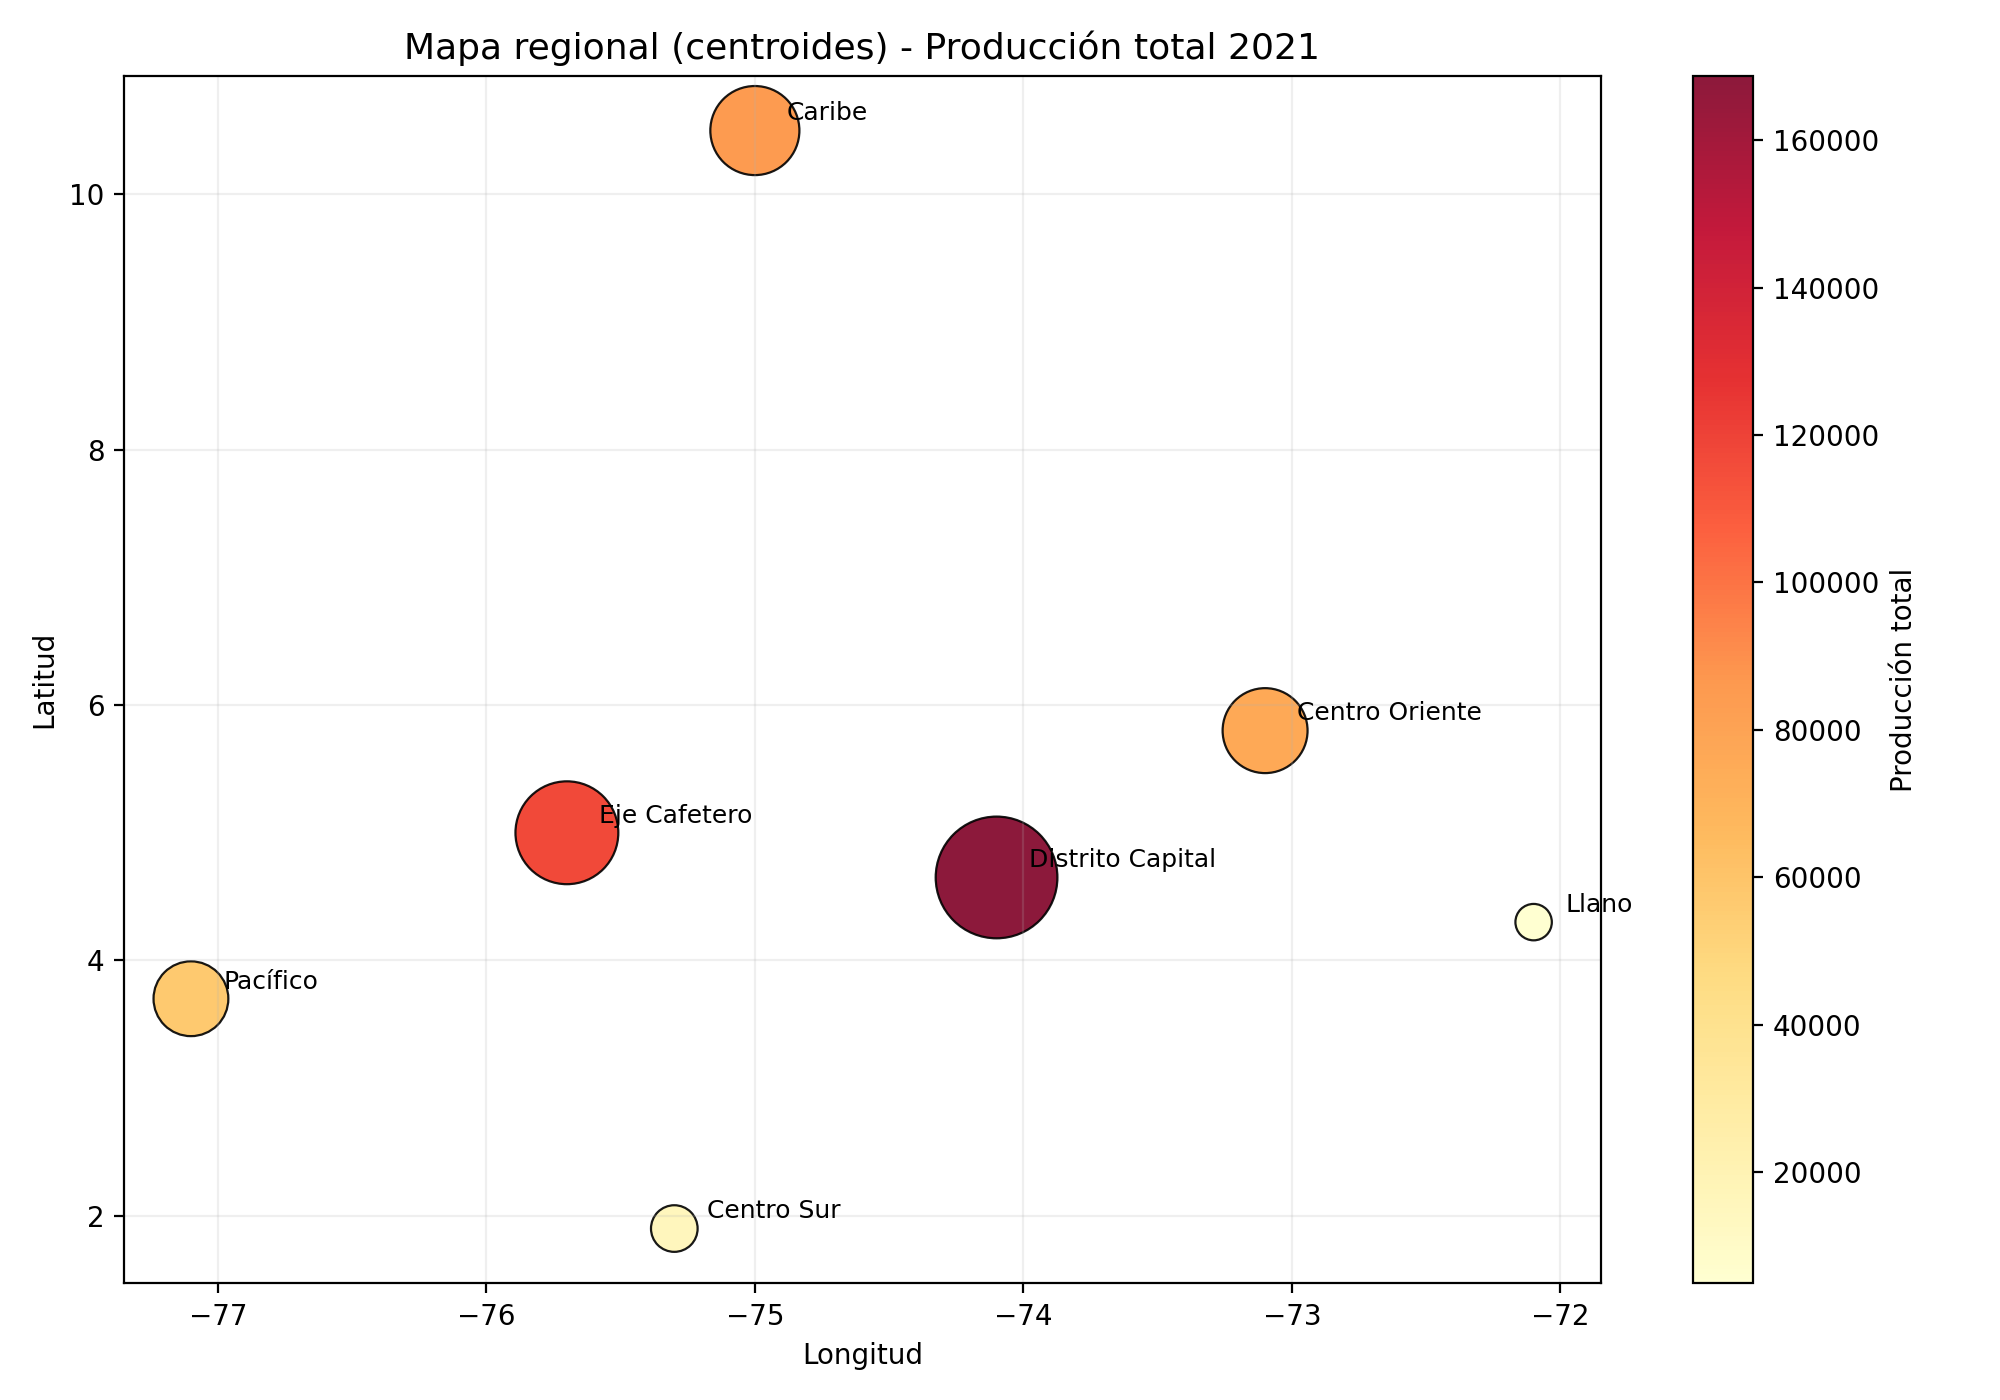
\includegraphics[width=0.88\textwidth]{dashboard_mapa_produccion_2021.png}
  \caption{Mapa regional por centroides para produccion total en 2021, consistente con la logica del dashboard\_streamlit\_v2.}
\end{figure}

\begin{figure}[H]
  \centering
  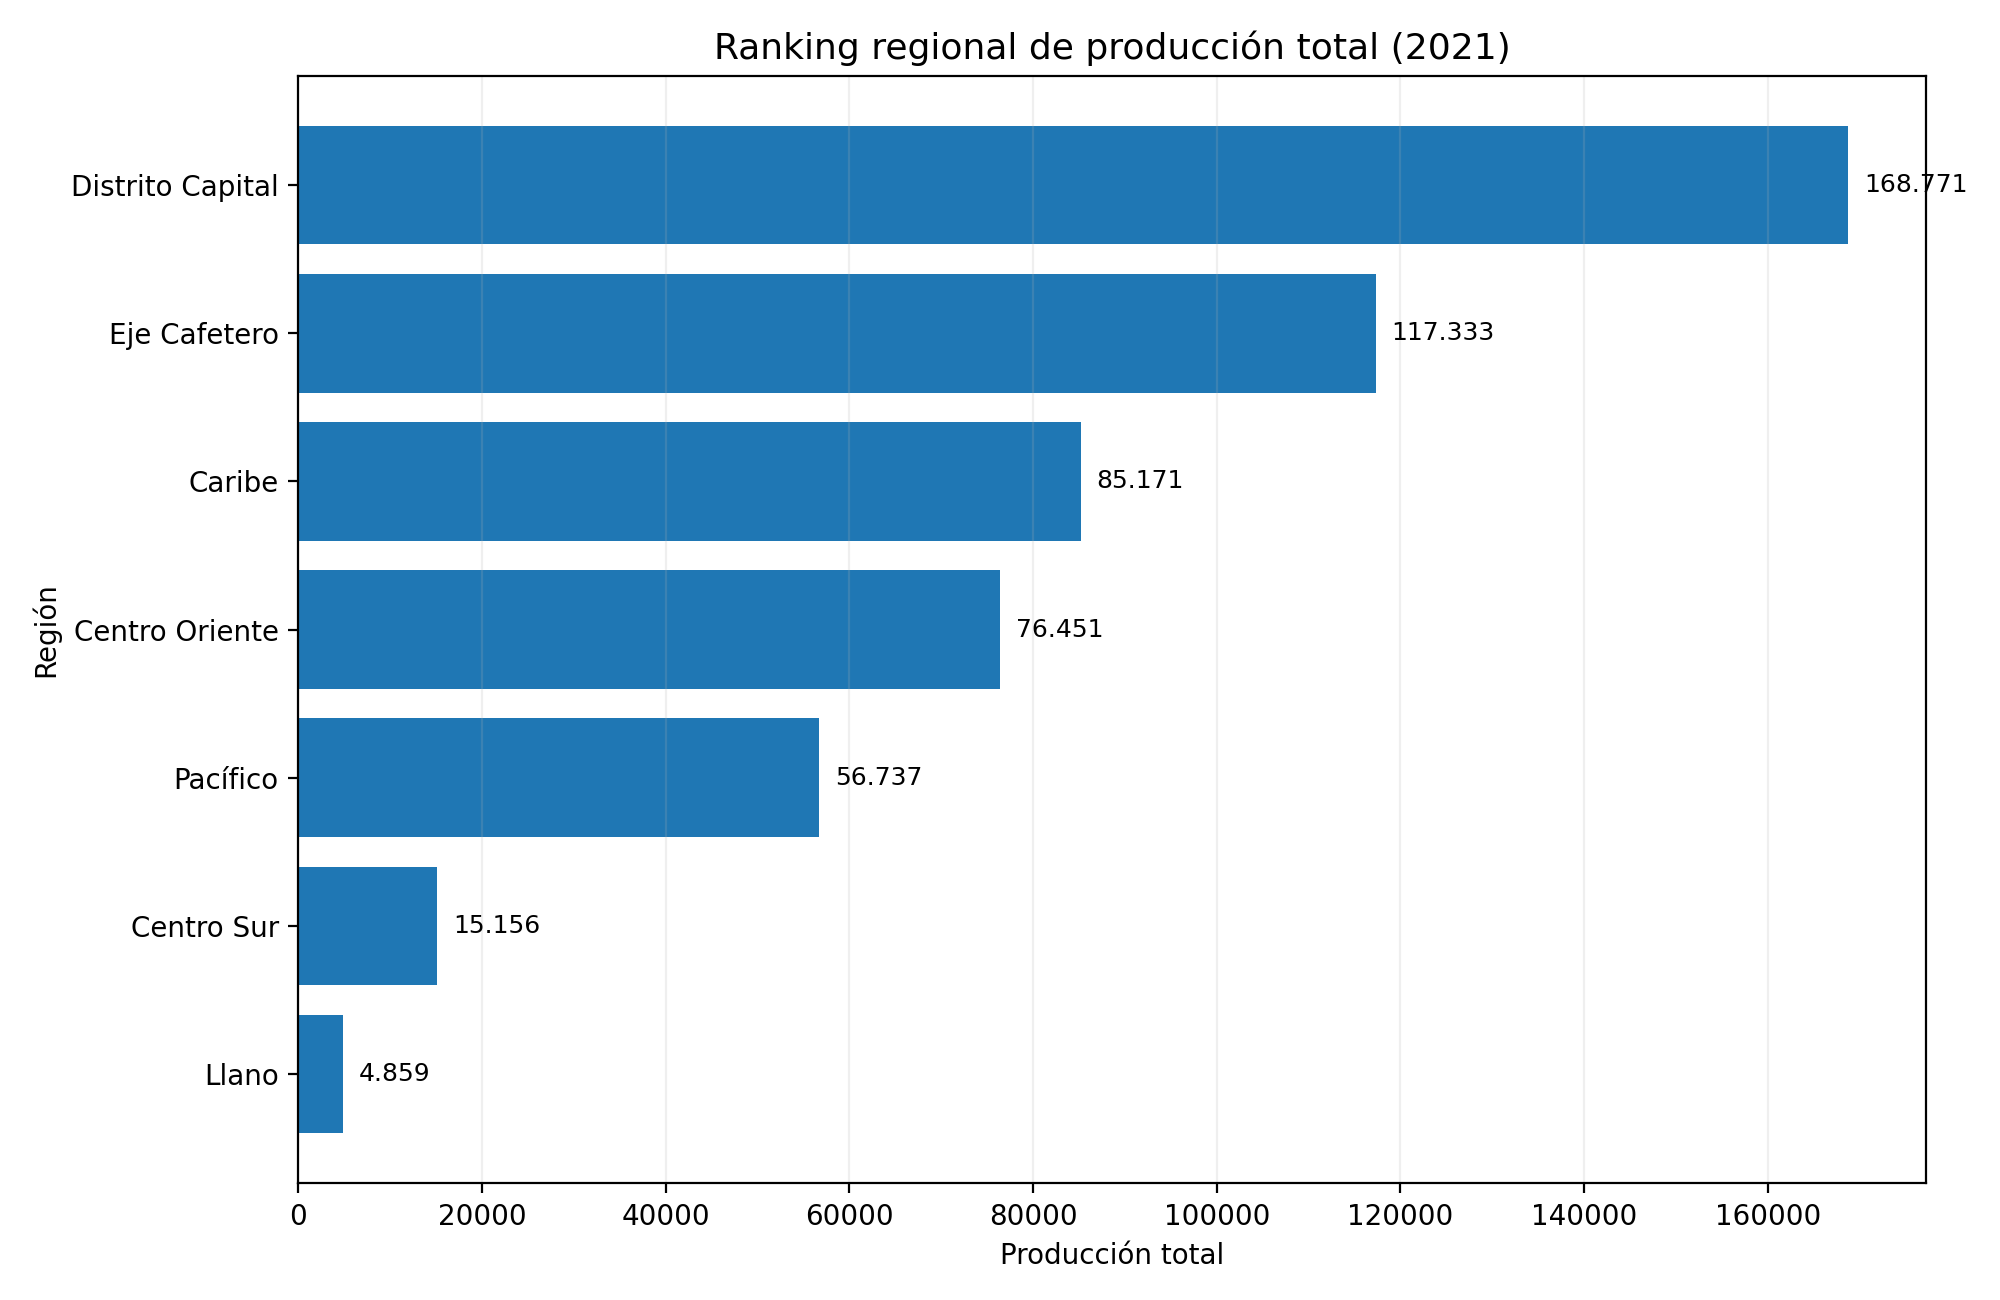
\includegraphics[width=0.88\textwidth]{dashboard_ranking_produccion_2021.png}
  \caption{Ranking regional de produccion total en 2021 derivado de los datos del dashboard.}
\end{figure}

Desde el punto de vista analitico, el mapa y el ranking muestran una concentracion espacial clara de la produccion en pocas regiones, mientras otras mantienen participaciones mas bajas. Esta evidencia refuerza la interpretacion del proyecto: los indicadores territoriales no solo describen volumen, sino que permiten identificar brechas regionales y orientar decisiones de politica cientifica con mayor precision.

Adicionalmente, la comparacion 2017-2019-2021 muestra una trayectoria de crecimiento acumulado del volumen total, pero con una estructura territorial relativamente estable en el grupo de regiones lideres. Esto sugiere que el sistema crece en magnitud, aunque conserva patrones de concentracion regional que merecen seguimiento en futuras convocatorias.

\section{Evidencia grafica del proceso}

Las siguientes figuras hacen parte de los artefactos del proyecto y se incluyen como evidencia del trabajo analitico que acompano el desarrollo del tablero.

\begin{figure}[H]
  \centering
  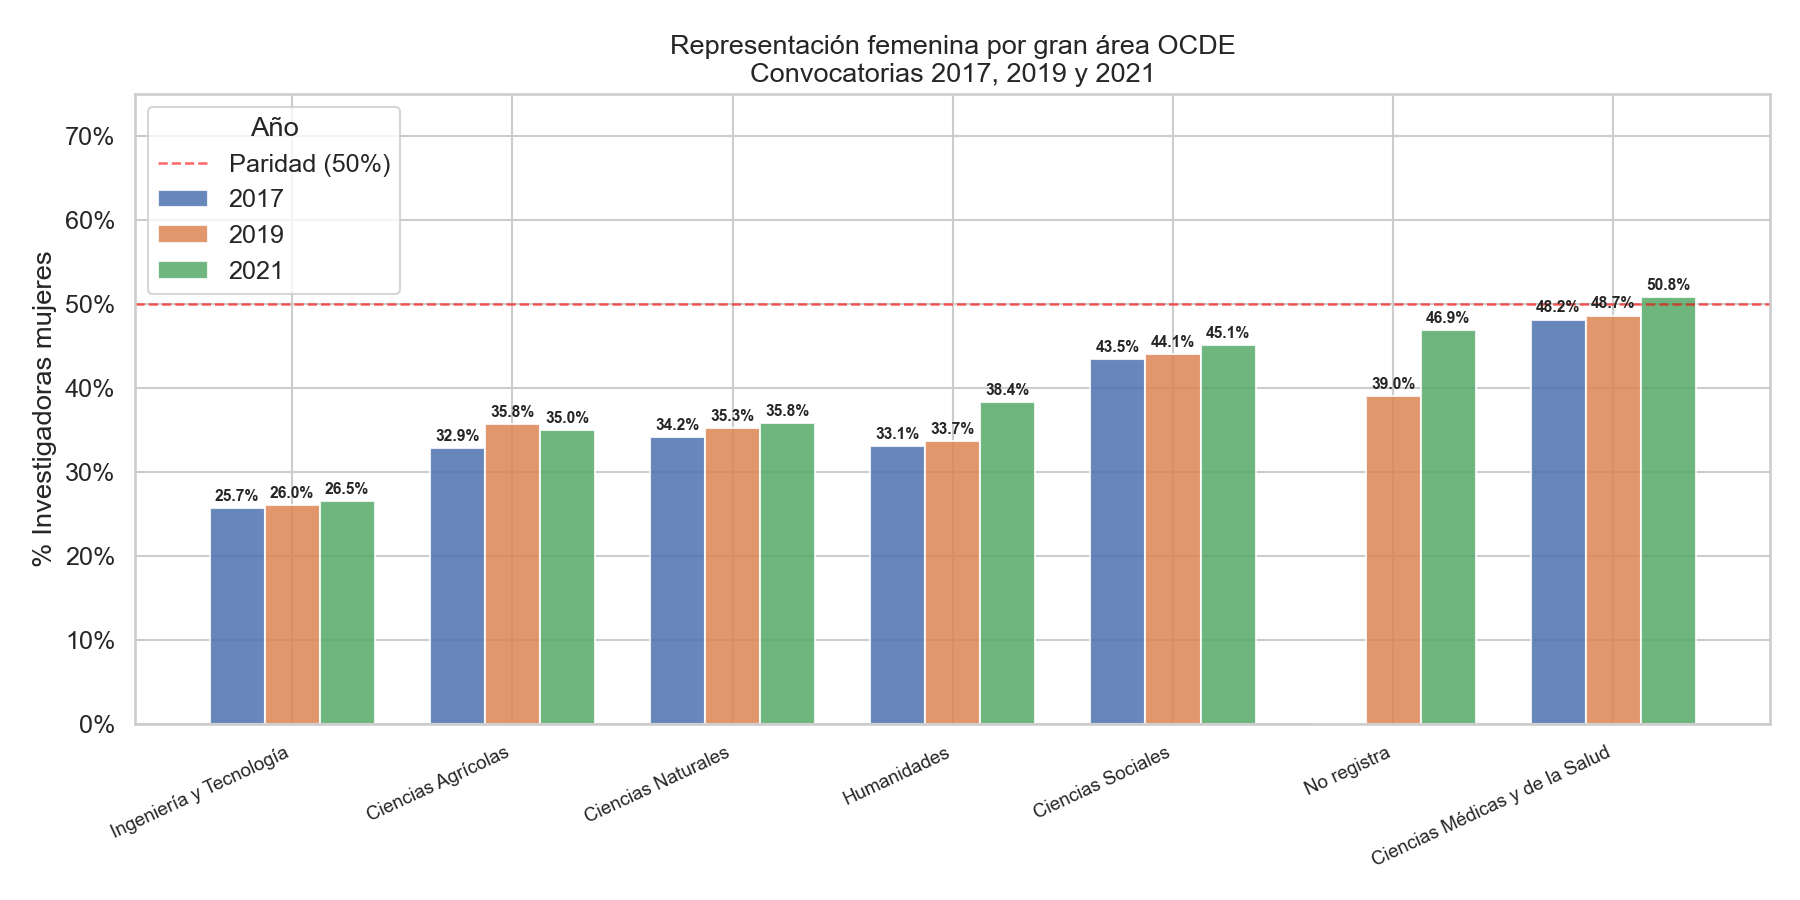
\includegraphics[width=0.9\textwidth]{fig1_barras_pct_femenino.png}
  \caption{Participacion femenina por gran area OCDE.}
\end{figure}

\begin{figure}[H]
  \centering
  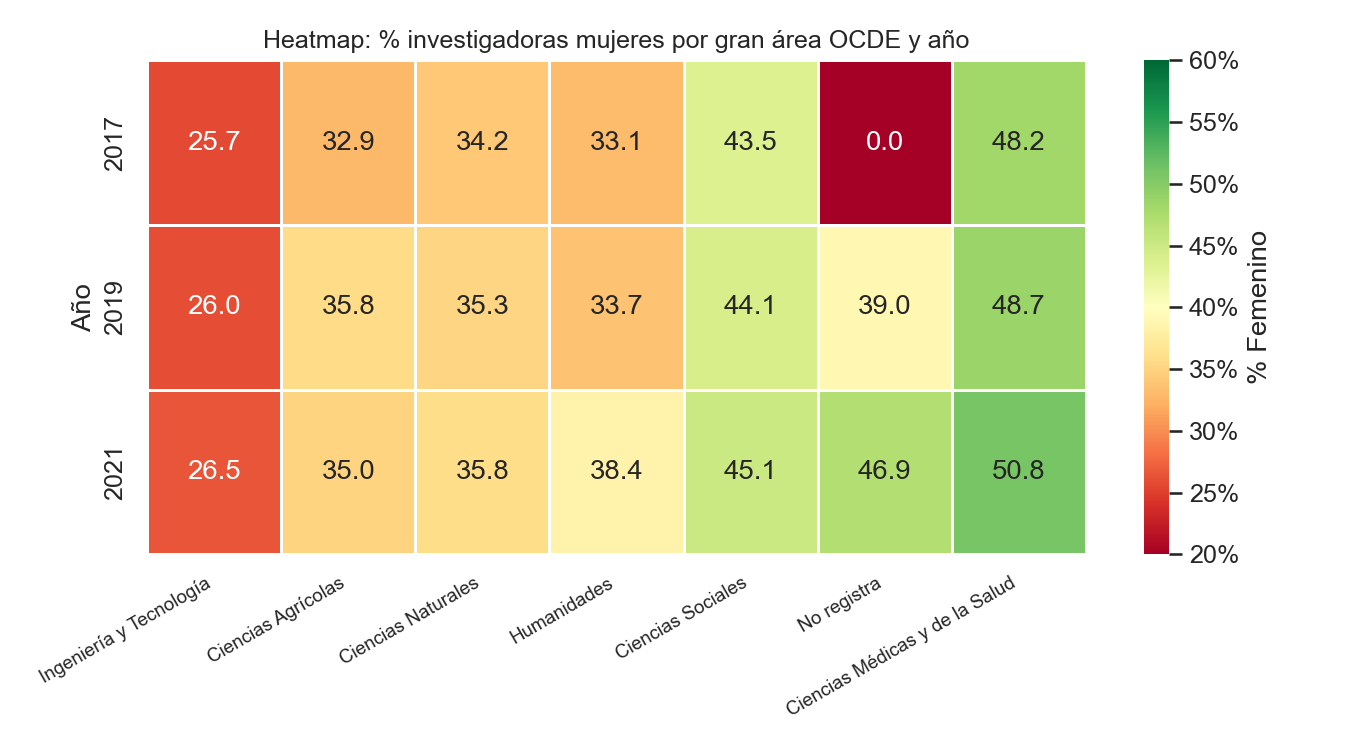
\includegraphics[width=0.9\textwidth]{fig2_heatmap_pct_femenino.png}
  \caption{Heatmap de participacion femenina por gran area y convocatoria.}
\end{figure}

\begin{figure}[H]
  \centering
  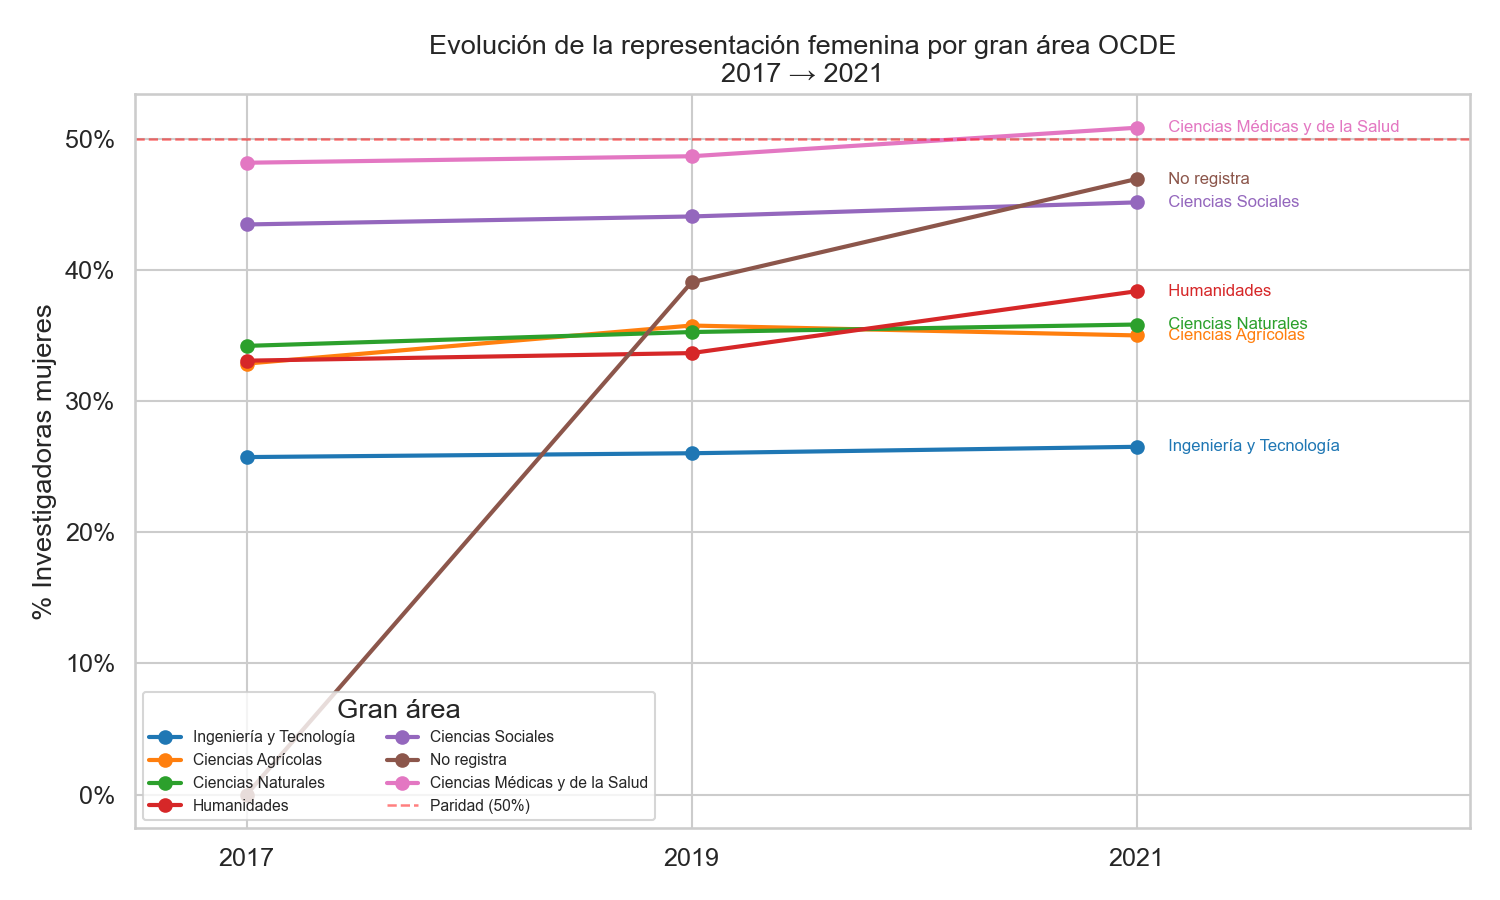
\includegraphics[width=0.9\textwidth]{fig3_lineas_evolucion.png}
  \caption{Evolucion temporal de participacion femenina.}
\end{figure}

\begin{figure}[H]
  \centering
  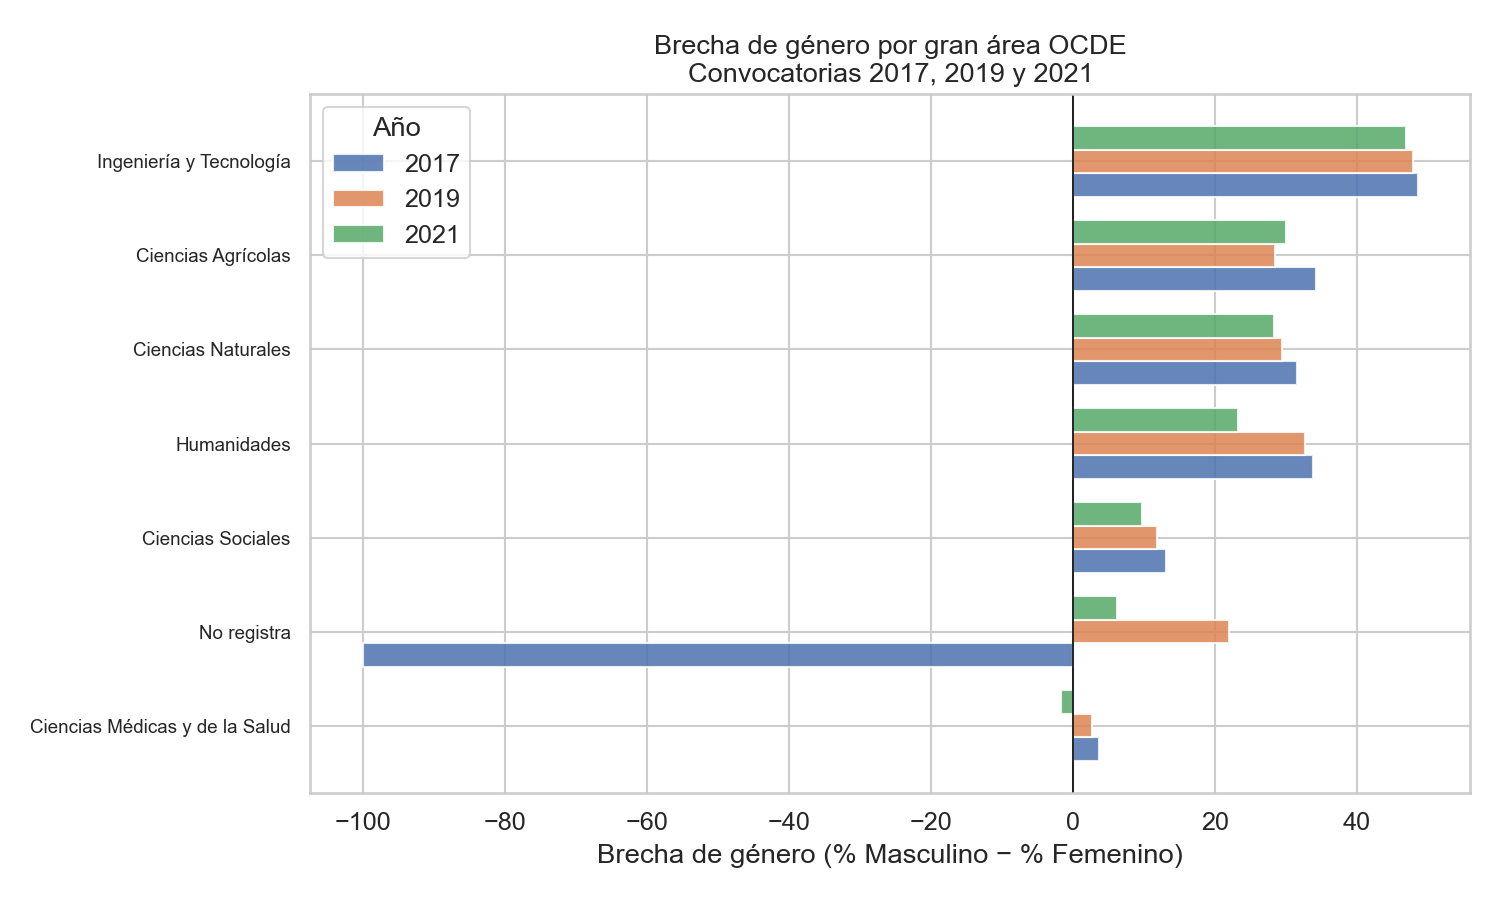
\includegraphics[width=0.9\textwidth]{fig4_brecha_genero.png}
  \caption{Brecha de genero por area de conocimiento.}
\end{figure}

\section{Discusion}

Un aporte importante del proyecto fue pasar de resultados dispersos a una salida integrada y util para consulta. Durante el proceso se evidencio que la calidad del analisis no depende solo de formulas de indicadores, sino tambien de decisiones de organizacion, trazabilidad y reproducibilidad.

La implementacion final demuestra que es posible mantener rigor tecnico y, al mismo tiempo, producir una visualizacion entendible para usuarios no tecnicos. El dashboard funciona como punto de llegada del proceso, pero su valor real esta en el trabajo previo de consolidacion y validacion de datos.

\section{Conclusiones}

\begin{enumerate}[label=\arabic*.]
  \item El proyecto se construyo de manera progresiva y con una secuencia de trabajo clara, desde organizacion de insumos hasta visualizacion final.
  \item La consolidacion de indicadores regionales permitio una lectura mas completa del comportamiento territorial de la produccion cientifica.
  \item El dashboard final quedo operativo para entorno web, sin dependencia de rutas locales, lo cual mejora la reproducibilidad.
  \item Los resultados confirman liderazgos regionales diferenciados segun el tipo de indicador, por lo que no es adecuado evaluar el desempeno solo con una metrica.
  \item El informe y la aplicacion quedan alineados sobre los mismos archivos de datos versionados, fortaleciendo la transparencia del proceso.
\end{enumerate}

\section{Recomendaciones}

\begin{enumerate}[label=\arabic*.]
  \item Mantener actualizada una carpeta unica de informe final con texto, imagenes y anexos para facilitar sustentaciones.
  \item Definir una rutina de actualizacion de indicadores cuando ingresen nuevas convocatorias.
  \item Incorporar capturas del dashboard en ejecucion como anexo visual complementario en la version final entregada al curso.
\end{enumerate}

\section{Referencias}

Departamento Administrativo Nacional de Estadistica. (2018). \textit{Censo Nacional de Poblacion y Vivienda 2018}. \url{https://www.dane.gov.co}

Departamento Administrativo Nacional de Estadistica. (2018). \textit{Encuesta Nacional de Calidad de Vida 2018}. \url{https://www.dane.gov.co}

Ministerio de Ciencia, Tecnologia e Innovacion. (s. f.). \textit{Investigadores reconocidos por convocatoria (2017, 2019, 2021)}. Datos Abiertos Colombia. \url{https://www.datos.gov.co/Ciencia-Tecnolog-a-e-Innovaci-n/Investigadores-Reconocidos-por-convocatoria/bqtm-4y2h/about_data}

Ustadistica. (2026). \textit{Observatorio MinCiencias - Investigadores Reconocidos}. GitHub. \url{https://github.com/ustadistica/Observatorio_Ministerio_de_Ciencias_Grupo7}

\end{document}
